% Préambule commun des schémas TikZ (compilés séparément par construire_figures.py)
\documentclass[tikz,border=3pt]{standalone}
\usepackage[T1]{fontenc}
\usepackage[utf8]{inputenc}
\usepackage{lmodern}
\usepackage{amsmath,amssymb}
\usepackage{bm}
\usepackage[american,siunitx,straightvoltages]{circuitikz}
\usetikzlibrary{arrows.meta,positioning,calc,decorations.pathmorphing,
  decorations.markings,decorations.pathreplacing,patterns,shapes.geometric,
  shapes.misc,shapes.multipart,fit,backgrounds,3d,intersections,matrix}

\ctikzset{bipoles/length=1.1cm, amplifiers/scale=0.85, tripoles/op amp/width=1.4}

\tikzset{
  >={Latex[length=2mm,width=1.4mm]},
  every picture/.style={line width=0.6pt, font=\small},
  % schémas-blocs
  bloc/.style={draw, minimum width=1.5cm, minimum height=0.9cm, align=center,
               inner sep=3pt, fill=white},
  somme/.style={draw, circle, minimum size=4.5mm, inner sep=0pt, fill=white,
                path picture={\draw (path picture bounding box.north west)
                  -- (path picture bounding box.south east)
                  (path picture bounding box.north east)
                  -- (path picture bounding box.south west);}},
  gain/.style={draw, isosceles triangle, isosceles triangle apex angle=60,
               minimum size=8mm, inner sep=1pt, fill=white},
  bruit/.style={draw, circle, minimum size=4.5mm, inner sep=0pt, fill=white,
                path picture={\node at (path picture bounding box.center)
                  {\scriptsize$\ast$};}},
  cadre/.style={draw, dashed, rounded corners=1pt},
  cadrept/.style={draw, dash dot, rounded corners=1pt},
  fleche/.style={->},
  % mécanique
  bati/.style={pattern=north east lines, draw=none},
  ressort/.style={decorate, decoration={coil, aspect=0.4, segment length=2.2mm,
                  amplitude=2mm, pre length=2mm, post length=2mm}},
  zigzag/.style={decorate, decoration={zigzag, segment length=2mm,
                  amplitude=1.6mm, pre length=2mm, post length=2mm}},
  pivot/.style={draw, circle, fill=white, minimum size=2.2mm, inner sep=0pt},
  masse/.style={draw, fill=gray!25, minimum width=1.4cm, minimum height=0.8cm},
  cote/.style={<->, line width=0.4pt},
  axe/.style={->, line width=0.6pt},
  trait mixte/.style={dash dot, line width=0.4pt},
}

% Encastrement / bâti hachuré : \bati{(x1,y1)}{(x2,y2)} trace une ligne et ses hachures dessous
\newcommand{\bati}[3][0.18]{%
  \fill[pattern=north east lines] #2 rectangle ($#3+(0,-#1)$);
  \draw[line width=0.8pt] #2 -- #3;}

% Transducteur (deux cercles entrelacés) : \pic (t) at (x,y) {transducteur};  -> (t-o) entrée, (t-e) sortie
\tikzset{
  transducteur/.pic={\draw (-0.13,0) circle (0.24); \draw (0.13,0) circle (0.24);
    \coordinate (-o) at (-0.37,0); \coordinate (-e) at (0.37,0);
    \coordinate (-n) at (0,0.24); \coordinate (-s) at (0,-0.24);},
  bobine/.style={decorate, decoration={coil, aspect=0.7, segment length=1.4mm,
                 amplitude=1.6mm, pre length=1mm, post length=1mm}},
  sourcebruit/.style={draw, circle, minimum size=5mm, inner sep=0pt, fill=white,
                 label={[inner sep=0pt]center:$\ast$}},
  sourcecourant/.style={draw, circle, minimum size=5mm, inner sep=0pt, fill=white,
                 label={[inner sep=0pt]center:$\circledast$}},
}

% Composants compacts (pour les petits boîtiers des schémas-blocs)
\newcommand{\resistance}[2]{% de #1 à #2 (quelconque)
  \draw #1 -- ($#1!0.22!#2$) ($#1!0.78!#2$) -- #2;
  \draw[decorate, decoration={zigzag, segment length=1.5mm, amplitude=1.1mm}]
    ($#1!0.22!#2$) -- ($#1!0.78!#2$);}
\newcommand{\condensateur}[2]{% horizontal de #1 à #2
  \draw #1 -- ($($#1!0.5!#2$)+(-0.05,0)$) ($($#1!0.5!#2$)+(0.05,0)$) -- #2;
  \draw[line width=1pt] ($($#1!0.5!#2$)+(-0.05,0.14)$) -- ($($#1!0.5!#2$)+(-0.05,-0.14)$)
                        ($($#1!0.5!#2$)+(0.05,0.14)$) -- ($($#1!0.5!#2$)+(0.05,-0.14)$);}
% R // C horizontal : \RparC{(x,y)}{longueur}{écart}  (centre, longueur totale, écart vertical)
\newcommand{\RparC}[3]{%
  \coordinate (rcA) at ($#1+(-#2/2,0)$); \coordinate (rcB) at ($#1+(#2/2,0)$);
  \draw (rcA) -- ++(0.15,0) coordinate (rcA1) (rcB) -- ++(-0.15,0) coordinate (rcB1);
  \draw (rcA1) -- ++(0,#3/2) (rcA1) -- ++(0,-#3/2) (rcB1) -- ++(0,#3/2) (rcB1) -- ++(0,-#3/2);
  \resistance{($(rcA1)+(0,#3/2)$)}{($(rcB1)+(0,#3/2)$)}
  \condensateur{($(rcA1)+(0,-#3/2)$)}{($(rcB1)+(0,-#3/2)$)}}

\begin{document}
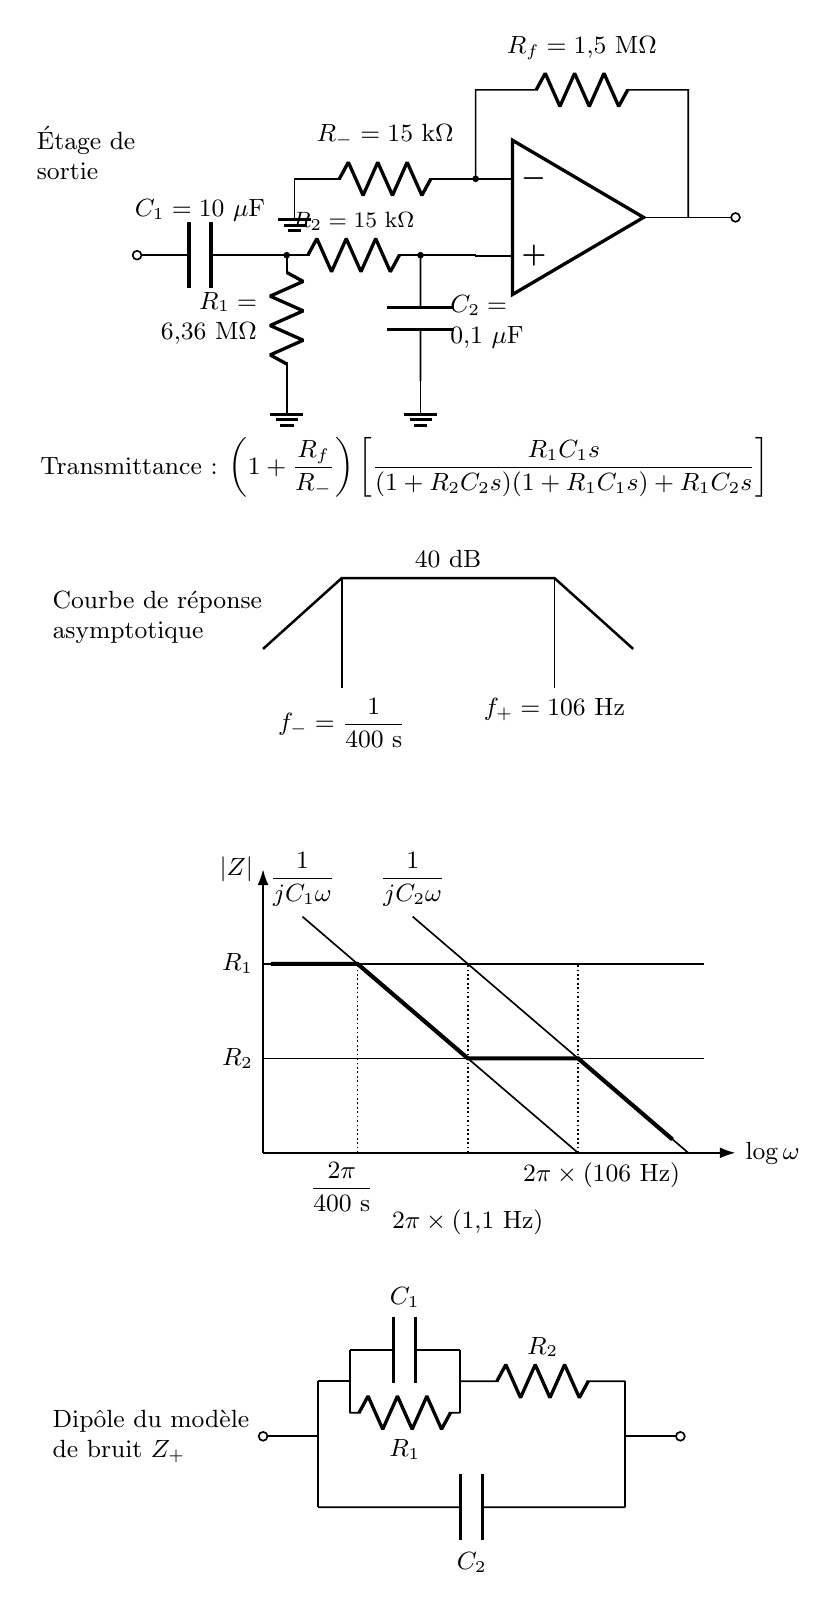
\begin{tikzpicture}[font=\small]
  % ---------- étage de sortie ----------
  \node[align=left, anchor=west] at (-1.4,1.3) {Étage de\\sortie};
  \draw (5.6,0.48) node[op amp, noinv input down] (a) {};
  \draw (0,0) node[ocirc] {} to[C] (1.6,0) -- (1.9,0);
  \node[above] at (0.8,0.3) {$C_1 = 10~\mu$F};
  \fill (1.9,0) circle (1.2pt);
  \draw (1.9,0) to[R] (1.9,-1.6) node[ground] {};
  \node[left, align=right] at (1.65,-0.8) {$R_1 =$\\$6{,}36$ M$\Omega$};
  \draw (1.9,0) to[R] (3.6,0);
  \node[above, font=\footnotesize] at (2.75,0.18) {$R_2 = 15$ k$\Omega$};
  \fill (3.6,0) circle (1.2pt);
  \draw (3.6,0) to[C] (3.6,-1.6) node[ground] {};
  \node[right, align=left] at (3.85,-0.85) {$C_2 =$\\$0{,}1~\mu$F};
  \draw (3.6,0) -- (4.3,0) |- (a.+);
  \draw (a.-) -- (4.3,0 |- a.-) coordinate (N);
  \fill (N) circle (1.2pt);
  \draw (N) to[R] (2.0,0 |- N) -- ++(0,-0.1) node[ground] {};
  \node[above] at (3.15,1.25) {$R_- = 15$ k$\Omega$};
  \draw (N) -- (4.3,2.1) to[R] (7.0,2.1) -- (7.0,0.48);
  \node[above] at (5.65,2.35) {$R_f = 1{,}5$ M$\Omega$};
  \draw (a.out) -- (7.6,0.48) node[ocirc] {};
  \node at (3.4,-2.7) {Transmittance : $\left(1+\dfrac{R_f}{R_-}\right)\left[\dfrac{R_1C_1s}{(1+R_2C_2s)(1+R_1C_1s)+R_1C_2s}\right]$};
  % ---------- réponse asymptotique ----------
  \begin{scope}[shift={(0,-5.2)}]
    \node[align=left, anchor=west] at (-1.2,0.6) {Courbe de réponse\\asymptotique};
    \draw[line width=0.9pt] (1.6,0.2) -- (2.6,1.1) -- (5.3,1.1) -- (6.3,0.2);
    \draw (2.6,1.1) -- (2.6,-0.3) (5.3,1.1) -- (5.3,-0.3);
    \node[above] at (3.95,1.1) {40 dB};
    \node[below] at (2.6,-0.3) {$f_- = \dfrac{1}{400~\text{s}}$};
    \node[below] at (5.3,-0.3) {$f_+ = 106$ Hz};
  \end{scope}
  % ---------- impédance |Z| ----------
  \begin{scope}[shift={(1.6,-11.4)}]
    \draw[->] (0,0) -- (6.0,0) node[right] {$\log\omega$};
    \draw[->] (0,0) -- (0,3.6) node[left] {$|Z|$};
    \draw (0,2.4) -- (5.6,2.4) (0,1.2) -- (5.6,1.2);
    \node[left] at (0,2.4) {$R_1$}; \node[left] at (0,1.2) {$R_2$};
    \draw (0.5,3.0) -- (4.0,0.0) (1.9,3.0) -- (5.4,0.0);
    \node[above] at (0.5,3.0) {$\dfrac{1}{jC_1\omega}$}; \node[above] at (1.9,3.0) {$\dfrac{1}{jC_2\omega}$};
    \draw[line width=1.5pt] (0.1,2.4) -- (1.2,2.4) -- (2.6,1.2) -- (4.0,1.2) -- (5.2,0.17);
    \foreach \x in {1.2,2.6,4.0} \draw[densely dotted] (\x,0) -- (\x,2.4);
    \node[below] at (1.0,0) {$\dfrac{2\pi}{400~\text{s}}$};
    \node[below=6mm] at (2.6,0) {$2\pi\times(1{,}1~\text{Hz})$};
    \node[below] at (4.3,0) {$2\pi\times(106~\text{Hz})$};
  \end{scope}
  % ---------- dipôle du modèle de bruit ----------
  \begin{scope}[shift={(0,-15.0)}]
    \node[align=left, anchor=west] at (-1.2,0) {Dipôle du modèle\\de bruit $Z_+$};
    \draw (1.6,0) node[ocirc] {} -- (2.3,0);
    \draw (2.3,0.7) -- (2.3,-0.9) (6.2,0.7) -- (6.2,-0.9);
    \draw (2.3,-0.9) to[C, l_=$C_2$] (6.2,-0.9);
    \draw (2.3,0.7) -- (2.7,0.7);
    \draw (2.7,1.1) to[C, l=$C_1$] (4.1,1.1); \draw (2.7,0.3) to[R, l_=$R_1$] (4.1,0.3);
    \draw (2.7,1.1) -- (2.7,0.3) (4.1,1.1) -- (4.1,0.3);
    \draw (4.1,0.7) to[R, l=$R_2$] (6.2,0.7);
    \draw (6.2,0) -- (6.9,0) node[ocirc] {};
  \end{scope}
\end{tikzpicture}
\end{document}
